% !TEX TS-program = pdflatex
% !TEX encoding = UTF-8 Unicode
% 
% This is a simple template for a LaTeX document using the "article" class.
% See "book", "report", "letter" for other types of document.
% 
\documentclass[11pt]{article} % use larger type; default would be 10pt
% 
% 
% 
%%% The "real" document content comes below...
\usepackage[utf8]{inputenc} % set input encoding (not needed with XeLaTeX)

%%% Examples of Article customizations
% These packages are optional, depending whether you want the features they provide.
% See the LaTeX Companion or other references for full information.

%%% PAGE DIMENSIONS
\usepackage{geometry} % to change the page dimensions
\geometry{a4paper} % or letterpaper (US) or a5paper or....
% \geometry{margin=2in} % for example, change the margins to 2 inches all round
% \geometry{landscape} % set up the page for landscape
%   read geometry.pdf for detailed page layout information

\usepackage{graphicx} % support the \includegraphics command and options

% \usepackage[parfill]{parskip} % Activate to begin paragraphs with an empty line rather than an indent

%%% PACKAGES
\usepackage{booktabs} % for much better looking tables
\usepackage{array} % for better arrays (eg matrices) in maths
\usepackage{paralist} % very flexible & customisable lists (eg. enumerate/itemize, etc.)
\usepackage{verbatim} % adds environment for commenting out blocks of text & for better verbatim
\usepackage{subfig} % make it possible to include more than one captioned figure/table in a single float
% These packages are all incorporated in the memoir class to one degree or another...

%%% HEADERS & FOOTERS
\usepackage{fancyhdr} % This should be set AFTER setting up the page geometry
\pagestyle{fancy} % options: empty , plain , fancy
\renewcommand{\headrulewidth}{0pt} % customise the layout...
\lhead{}\chead{}\rhead{}
\lfoot{}\cfoot{\thepage}\rfoot{}

%%% SECTION TITLE APPEARANCE
\usepackage{sectsty}
\allsectionsfont{\sffamily\mdseries\upshape} % (See the fntguide.pdf for font help)
% (This matches ConTeXt defaults)

%%% ToC (table of contents) APPEARANCE
\usepackage[nottoc,notlof,notlot]{tocbibind} % Put the bibliography in the ToC
\usepackage[titles,subfigure]{tocloft} % Alter the style of the Table of Contents
\renewcommand{\cftsecfont}{\rmfamily\mdseries\upshape}
\renewcommand{\cftsecpagefont}{\rmfamily\mdseries\upshape} % No bold!

%%% END Article customizations
\usepackage{xcolor}
\usepackage{tcolorbox}
\usepackage{lipsum}  % 示例文本
\usepackage{mdframed}

\usepackage{tikz}

% 
\title{Introduction to Mathematics for Data Science \\ Personal Assignnment 1}
\author{Zehao Qian}
\begin{document}
\maketitle
% 
% 
% 
\section{Question 1}
\subsection{Modelling Bird Population Decline Due to Invasive Snakes}
% 
\paragraph{To model the bird population over time until extinction, I use a logistic growth model, which is commonly used to describe population growth and decline. The logistic growth model is expressed as:}
% 
\[P(t) = \frac{K}{1 + \frac{K - P_0}{P_0} \cdot e^{-rt}}\]
% 
\paragraph{Where:}
\begin{itemize}
    \item \(P(t)\) is the population at time \(t\).
    \item \(K\) is the carrying capacity, representing the maximum sustainable population size.
    \item \(P_0\) is the initial population at \(t = 0\).
    \item \(r\) is the growth rate parameter.
    \item \(t\) is time.
\end{itemize}
% 
% 
\paragraph{In your scenario, the bird population is declining due to the invasive snake species, so you'll need to use a negative growth rate (\(r < 0\)). The population starts at a certain level (\(P_0\)) and gradually approaches zero as time progresses.}

\paragraph{Here's a Python function that models the bird population over time using the logistic growth model and plots it:}
% 
% 
\begin{figure}[H]
    \centering
    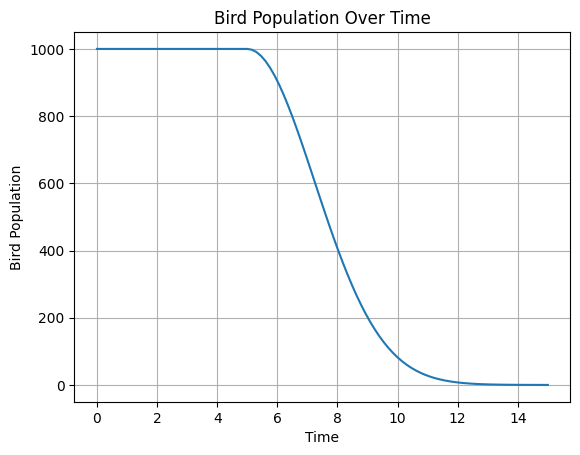
\includegraphics[width=0.75\textwidth]{pic/BirdPopullationModel.png}
    \caption{Bird Prediction Graph}
\end{figure}
% 
% 
\end{document}
% 